%!TEX root = ../template.tex
%%%%%%%%%%%%%%%%%%%%%%%%%%%%%%%%%%%%%%%%%%%%%%%%%%%%%%%%%%%%%%%%%%%%
%% chapter3.tex
%% NOVA thesis document file
%%
%% Chapter with iCBD project
%%%%%%%%%%%%%%%%%%%%%%%%%%%%%%%%%%%%%%%%%%%%%%%%%%%%%%%%%%%%%%%%%%%%


%%-------------------------------------------------------------------
%%	3 - iCBD - Infrastructure for Client-Based (Virtual) Desktop (Computing)
%%-------------------------------------------------------------------
\chapter{iCBD - Infrastructure for Client-Based Desktop}
\label{cha:icbd}

The acronym \gls{iCBD} stands for Infrastructure for Client-Based (Virtual) Desktop (Computing). Is a platform being developed by an R\&D partnership between \textit{NOVA LINCS}, the Computer Science research unit hosted at the \textit{Departamento de Informática of Faculdade de Ciências e Tecnologia of Universidade NOVA de Lisboa} (DI-FCT NOVA) and \textit{SolidNetworks – Business Consulting, Lda} part of the \textit{Reditus S.A.} group. 

The primary goal is to implement a client based VDI, a specialised form of \gls{VDI} infrastructure, where client's computations are performed directly on the client hardware as opposed to performed on big and expensive servers. With the distinctive characteristic of not having the necessity of investing in hard disks for the client devices, as well as hoping to solve prominent predicaments in the administration and management of large-scale computer infrastructure.

This chapter will address the central concepts and associated technologies encompassed in this project, particularly:

\begin{description}
	%
	\item [Section~\ref{sec:icbd_concept}] overviews the core concepts of the project and particularly note the limitations and peculiarities of current implementations in contrast with the chosen approach.
	%
	\item [Section~\ref{sec:icbd_architecture}] studies the main architectural components of the platform, with emphasis on the different layers and how  they act together to serve the end-user.
\end{description}
\newpage


%%-------------------------------------------------------------------
%%	3.1 - The Concept
%%-------------------------------------------------------------------
\section{The Concept} % (fold)
\label{sec:icbd_concept}

The iCBD as a project aims to investigate an architecture that leads to the development of a platform that is similar to a client-based VDI, while maintaining all the benefits of both client-based and server-based VDI. Additionally, it should present the power of working as a Cloud \gls{DaaS} without any of the bad traits of the approaches as mentioned earlier.

The aim is to preserve the convenience and simplicity of a fully centralised management platform for Linux and Windows desktops, instantiating those in the users physical workstation from virtual machine templates (VMs) kept in repositories. We will further address this subject in section \ref{sec:icbd_architecture}\\

To summarise the platform should be able to:

\begin{itemize}
	\item Adapting to a wide range of server configurations, without prejudice to the defined architecture.
	%
	\item Minimize disruption in the use of workstations for end-users, offering a work environment and experience of use so close to the traditional one, that they should not be able to tell it from a standard local install.
	%
	\item Simplify installation, maintenance and platform management tasks for the entire infrastructure, including servers in their multiple roles, storage and network devices, all from a single point of administration.
	%
	\item Allow for a highly competitive per workstation cost.
	%
	\item Maintain an inter-site solution to efficiently support, e.g., a geographically disperse multi-site organisation.
\end{itemize}


%%-------------------------------------------------------------------
%%	3.2 - The Architecture 
%%-------------------------------------------------------------------
\section{The Architecture} % (fold)
\label{sec:icbd_architecture}

%Topics:
%Introduce the layers
%Draw a diagram 
%Layers are a kind of role, not a single a defined service but a collection 

The iCBD platform encompasses the use of multiple services. To achieve a better understanding of its inner workings, we can group these services in four major architectural blocks as seen in  figure~\ref{fig:icbd_layers}.


\begin{figure}[htbp]
	\centering
	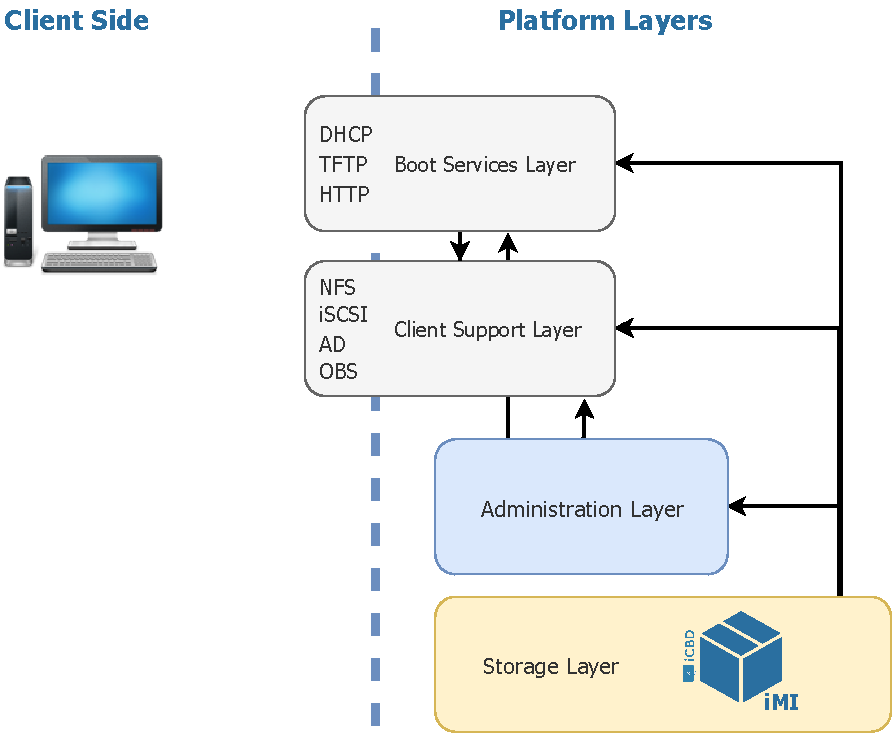
\includegraphics[height=4in]{cap3_iCBD_Layers}
	\caption{iCBD Layers View}
	\label{fig:icbd_layers}
\end{figure}


\begin{description}
	\item [\acrfull{iMI}] embodies the required files to run a iCBD platform client; this nomenclature was borrowed and adapted from Amazon Web Services AMI~\cite{aws_ami}. An iMI includes a VM template (with an operating system, configurations and applications), the iCBD boot package ( a collection of files needed for a network boot and custom-made to the operating system) and an assortment of configurations for services like PXE and iSCSI.
	%
	\item [Boot Services Layer] is responsible for providing the initial process from which the client machines will boot from the network, and later on transfer a bespoke boot package, using services such as \acrshort{PXE}, \acrshort{DHCP}, \acrshort{TFTP} and \acrshort{HTTP}.
	%
	\item [Administration Layer] to maintain all the iMI life cycle, from its creation to its retirement, currently this is done with a custom set of scripts.
	% takes advantage of a virtualisation stack (can be based in either \acrshort{KVM} or VMWare products) to engage in maintaining all the needed aspects for the successful creation and update processes of an \acrshort{iMI} lifecycle.  Employing a custom set of scripts, the creation of an iCBD Boot Package is also a duty of this layer. 
	%
	\item [Client Support Layer] provides support for client side operations including, e.g., authentication, read/write storage space for the client (since iMIs run on "diskless" workstations) and its home directories. 
	%deals with the demands of a deployed and running iCBD image, such as, providing read/write space (since iMIs run on diskless workstations) and storing users home directories. As well as, hosting domain controllers, centralised authentication amongst other services that can be already in place in the midst of a clients infrastructure. Granting the ability to deploy a customised iMI in any scenario.
	%
	\item [Storage Layer] maintains the repository of iMIs and provides essential operations such as version control of the VM images files. Our work is fundamentally focused on this layer, extending it in such a way that a single repository abstraction is built on top of the local / individual repositories through replication and caching. These local repositories are implemented on BTRFS or CEPH and may be exported to clients using \acrshort{NFS} or \acrshort{iSCSI}.
	
	%Is also in this layer that we seize the potential of replication features provided by the file systems employed. In this project, the storage relies on two mainstream file systems: BTRFS and CEPH. Together with services like \acrshort{NFS} and \acrshort{iSCSI} enables a way to export data to clients.
\end{description}
 
In the next subsections we will provide a more detailed description of each of the above-mentioned layers.

%%-------------------------------------------------------------------
%%	3.2. - iCBD Machine Image 
%%-------------------------------------------------------------------
\subsection{iCBD Machine Image}
\label{sub:icbd_imi}

\begin{figure}[htbp]
	\centering
	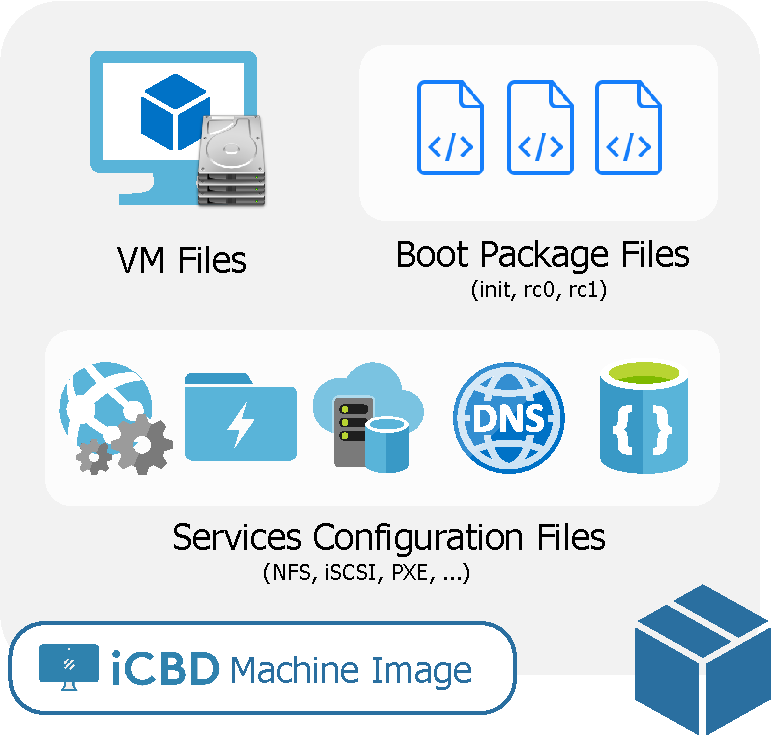
\includegraphics[height=4in]{cap3_iMI}
	\caption{iCBD Machine Image Files}
	\label{fig:icbd_iMI_files}
\end{figure}

In its essence, an iCBD Machine Image is the aggregation of everything that is needed to run an Operating System within the iCBD platform - data and configuration files. For the sake of simplicity, we categorise the files in three main groups.

\begin{description}
	\item [VM Template files] The main component is the virtual machine template in the form of a read-only image. As described in section~\ref{sub:res_vm_storage} the anatomy of a template follows the standard VMware and KVM formats either with multiple files (i.e., Virtual Disk Files like \texttt{.vmdk} or \texttt{.qcow}) or a \textit{raw} storage format.
	%
	\item [iCBD Boot Package files] In a network boot environment, such as the one used, there is a need to keep a set of files that manage the boot process of a workstation; these files can be included in the initial \textit{ramdisk} or later transferred over HTTP when needed. Included are an init file and at least two Run Control Script files (\texttt{rc0} and \texttt{rc1}) that are responsible for starting network services, mount all file systems and ultimately bring the system up in to the single-user level. With a tool such as \textit{BusyBox} (a single executable file with a stripped-down set of tools), a basic \textit{shell} is available during the boot process to fulfil all the required steps.
	%
	\item [Service Configuration files] Among the services that support iCBD, some do need changes in the configuration files. As an example, the "NFS exports" configuration file should reflect which file systems are exported, which networks a remote host can use, as well as a myriad of options that NFS allows to be set. The same happens to iSCSI, where an iSCSI target needs to refer to a backing store for the storage resource where the image resides. 
\end{description}

%\subsubsection{iMI Life Cycle}
\paragraph{iMI Life Cycle}
\label{subsub:icbd_imi_lifecycle}
The life cycle of an iMI encompasses all stages that take it throughout its course within the platform, Figure~\ref{fig:icbd_iMI_lifecycle} shows the major ones. From creation, through live deployment in use by multiple clients, and finally its decommission and placement in to temporary or cold storage.

\begin{figure}[htbp]
	\centering
	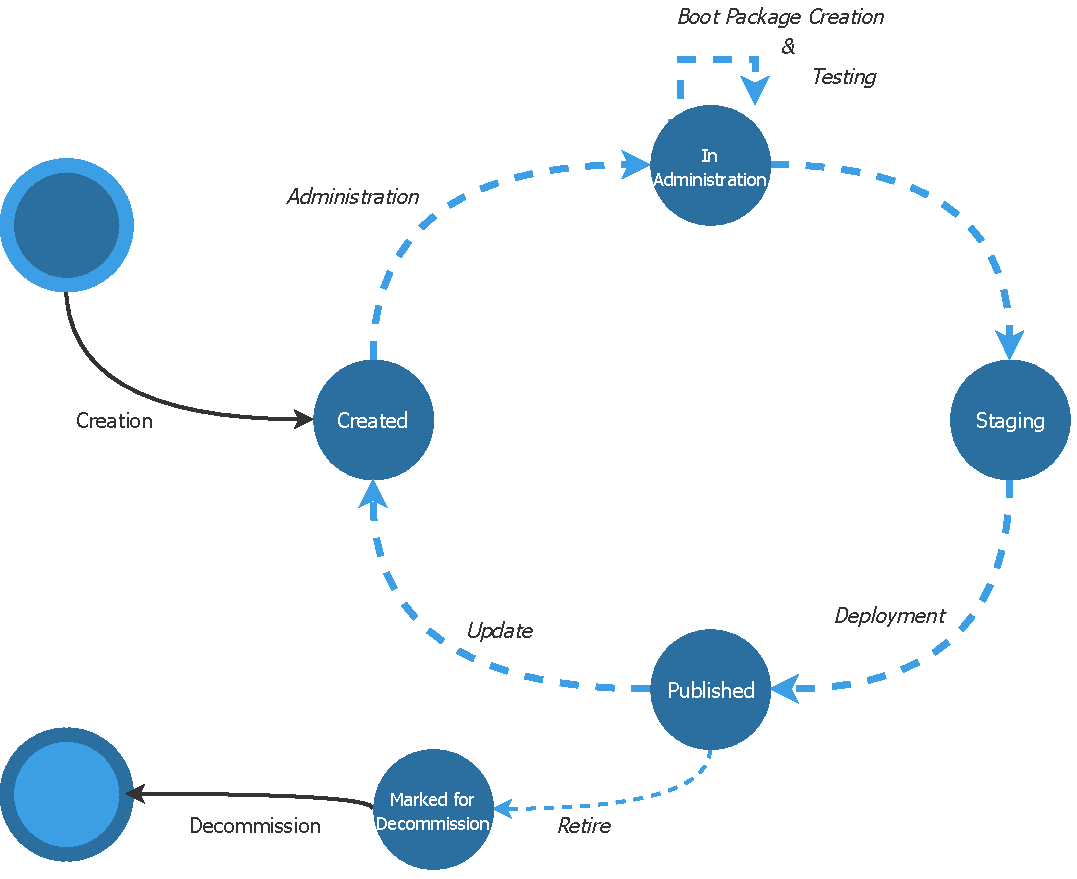
\includegraphics[height=4in]{cap3_iMI_Lifecycle}
	\caption{iMI Life Cycle inside the iCBD Platform}
	\label{fig:icbd_iMI_lifecycle}
\end{figure}

Each lap in the cycle is considered a new version. So every new update made to an iMI will spawn a new version. Through the snapshotting features of the storage layer, the creation of a new version is a rather straightforward and a computationally light operation.

During its life in the platform, an iMI can present it self into four main states:

\begin{description}
	\item [Created] After being inserted into the platform, an image is not instantaneously  ready to be served to clients and booted in a workstation; it must pass through a number of administration steps for the generation of a boot package.
	%
	\item [In Administration] An iMI goes through this phase in two moments: the first one, described above, where an image has just been injected into the platform. And the second and most frequent case, where an image needs to be updated or any way modified. 
	%It is here in this state that in interaction with the administration layer provides with a way to administer and update an iMI. 
	The iMI will stay in this state as long as it is being managed (which can take from a few minutes to hours). At the end this process the boot package is automatically created.
	% TODO Cap3 - FICAMOS AQUI NA REVISAO
	\item [Not Published] This status symbolises that the image is ready to work but isn't yet published and so not visible to platform users. This phase holds a particular interest in the testing the iMI for the correctness in the boot process and to ensure that the modifications were applied. Only after the testing procedures should an iMI made available for general use.
	%
	\item [Published] The stage where the iMI is expected to spend most of its time. One can think o   f this state as the proceeding into production of an iMI. After all the previous steps it is anticipated that the image is entirely ready to be delivered to the clients. At this stage, the platform in its Boot Services Layer announces to clients the possibility of choosing this image and provides the necessary support to its execution. Clients can instantiate the iMI as they please, taking advantage of the fact that can access their data and applications from nearly any device.
\end{description}

When an iMI completes a cycle and undergoes an update process, the old version is retired and goes to a fifth state, denominated \textbf{Marked for Decommission}, which is comparable to a stay in limbo. First, because when the administration process has initiated the probability of having clients using the image is significant, therefore the iMI needs to continue available for those clients. Even when the administration process ends, some client may still be using the image's old version. Thus only after all the clients cease utilising the iMI, can the image be transferred to its final state - \textbf{Decommission}. At this point, the version can be removed entirely from the platform or more wisely stored as a backup for some eventual failure in the future, or even if the administrator wants to recover an older state of the image.






%%-------------------------------------------------------------------
%%	3.2. - Boot Layer 
%%-------------------------------------------------------------------
\subsection{Boot Services Layer}
\label{sub:icbd_boot_layer}
% https://opensource.com/article/18/1/analyzing-linux-boot-process
% https://www.ibm.com/developerworks/library/l-linuxboot/index.html
% https://utcc.utoronto.ca/~cks/space/blog/linux/LinuxBootOverview?

From an end-user perspective, the only layer that is visible and interactive is the boot layer. The interface is lean and provides a way to select the image to boot in the workstation, however not every single aspect is noticeable. In the background, there is a need to resort to multiple services for starting a client's workstation with an iCBD Machine Image.

The platform provides two processes to remote boot an iMI. One instantiates, from an iMI, the Operating System natively on the bare metal workstation in the fashion of a standard diskless network boot. The other uses the above mechanism for provisioning a minimal iMI that was a hypervisor installed and virtualises any other iMI available in the storage layer. Both approaches are entirely transparent to the final user that does not grasp the differences and doesn't know if the working OS is virtualised or running natively.

The first part of the boot process starts like any other network boot, where a series of DHCP requests are used to provide the suitable client network parameters and particularly the location (IP address) of the TFTP server. Then begins the transference of a small network boot manager program. In this traditional PXE boot environment, a friendly looking tailored made graphical menu displays to the user an assortment of choices that announce the different iMIs ready to boot.

%\subsubsection{Booting an iMI in a Workstation }
\paragraph{Booting an iMI in a Workstation}
\label{subsub:icbd_booting_imi}
%(REF https://www.ibm.com/developerworks/library/l-initrd/index.html)
After the selection of an iMI in the PXE boot menu~\cite{ibm_linux_boot} the second-stage boot kicks in. Using \textit{PXELINUX} as a bootloader there is the capability of transferring a compressed Linux Kernal (vmlinuz) and an initial ramdisk (initrd) (REF in comment)through either TFTP or HTTP, is also in this step that some parameters needed during the boot are set with the correct values according to the image picked. After everything loaded into memory, the stage 2 boot loader invokes the kernel image, and after booted and initialised, the kernel starts the first user-space application. 

Commonly the first application is called init, and in the particular case of this platform, the init file starts the chain execution of other custom files (\texttt{rc0} and \texttt{rc1}). Those Run Control scripts configure every single aspect in the Operating System according to the characteristics of physical machine booting. The first step is to reconfigure the network card and obtain connectivity. Then, is determined if there is the need for getting more files indispensable for the remaining boot process if this need exists, then the missing files are transferred. The next script, \texttt{rc0}, deals with data volumes and their mounting method (i.e. r/w space, users home directories); in case of using the loading OS as a base for another iMI in virtualisation, some configurations are anticipated and applied. The file system of the underlying iMI is checked to verify if happens to be BTRFS or any other, in the case where BTRFS is adopted the Seeding capability comes into play in this step. After every aspect from the configuration is setup the \texttt{switch root} command is deployed moving the already mounted \texttt{/proc}, \texttt{/dev}, \texttt{/sys}, \texttt{/tmp} and \texttt{/run} to new root and makes this the new root filesystem.

At last, the residual configuration entails the update of the correct time with the NTP service and some last logging of statistics such as the elapsed time of the boot process and the bandwidth used by the sum of all operations.



%%-------------------------------------------------------------------
%%	3.2. - Administration Layer 
%%-------------------------------------------------------------------
\subsection{Administration Layer}
\label{sub:icbd_adm_layer}

One of the most important features provided by the platform, and personified in this next layer, is the ability to perform administration operations on an iMI. That task becomes simplified by the use of a provided image administration tool. Armed with such a mechanism any systems administrator in an organisation can make the changes that understand necessary (stuff like Operating System and software in general updates, add new software, modify configurations) and then publish the image in the platform for widespread use. 

%\subsubsection{The Administration Process}
%\label{subsub:admin_imi}

%\textbf{The Administration Process}
\paragraph{The Administration Process}
\label{par:admin_imi}
The administration tool consists of a series of scripts triggered by the main one called \texttt{adm}. Calling this script with the name of one iMI sets off the startup of a VM in a VMware ESXi server with a base image that will support the administration process. Commonly the OS used will be some flavour of Linux (Fedora 27, CentOS 7 or even Ubuntu 16.04 LTS).

The whole process makes extensive use of the snapshotting capabilities of the Storage Layer (whether using BTRFS or CEPH), with no prejudice to the complete system performance. For each iMI, there is a snapshot with an index number that relates to its version and age (i.e. the higher the number the most recent the version is). Multiple versions of an iMI persist stored in directories named by the index of the version. So, is simple to create a new linked clone from the most recent version.

The administration VM, after its boot process, will start a hypervisor (VMware Workstation or KVM) that in turn will get a new linked clone of the most recent version of the iMI to administrate. In this sense, this process makes use of nested virtualisation to achieve its goal, which can result in some slowness (even considering the use of a Type 1 hypervisor), but in theory, all the operations to the new snapshot could be performed on a physical machine using only one level of virtualisation. 
%(ref: https://www.linux-kvm.org/images/3/33/02x03-NestedVirtualization.pdf)
In this step, the snapshot that is in the management process is in a working directory, a temporary storage area with a limited lifetime to the duration of the procedure. This method serves two proposes. First, all the clients that are using the latest version of the iMI can remain using it with an administrative process running in parallel. The second is the ability to quickly discard all the changes made in the working directory in case of unwanted changes.

Finishing the process, with all the desired actions performed in the iMI, the administrator gets to chose between saving the changes done or discarding them. When choosing to proceed with saving the new version of the image, a process starts by changing the working directory to a permanent one, through a new linked clone of the working snapshot but this time following the naming system so that the version number will name the directory.


%\subsubsection{Creating the boot package}
%\label{subsub:createboot_imi}

\paragraph{Creating the boot package}
\label{par:icbd_create_bootpack}
Even after all the process described above, the iMI is not ready to boot, being the next step the creation of the boot package. This phase is the responsibility of the \texttt{mki} script which can be called immediately at the end of the administration process by the texttt{adm} tool depending on the type of the iMI.
The procedure is different for each type of iMI (Windows or Linux), but with a set of steps in common, being that the Linux iMIs requires a particular number of customisations. The peculiarity of these requirement comes from the fact that Linux iMIs can run natively on a client workstation serving as host for other images. Which in turn entails the creation of custom \texttt{initramfs} and \texttt{vmlinuz} files, the addition of Kernel drivers and firmware, the tailor-making of Run Control Scriptfiles (rc0 and rc1) that start the network services with a configuration compatible with the platform and mount the correct remote file systems. In the end, is also added a script called \texttt{runvm}, that is instrumental in managing the launch of a virtualised iMI, as well as configure the hypervisor parameters to take the best advantage of the client hardware.
However, there is more to the \texttt{mki} script. For both flavours of the iMIs, the configurations of the \textit{iSCSI targets} need an update to reflect the new version of the iMI, with the same happening to the \textit{pxelinux} configuration that requires the new paths to the files served to the clients.


%%-------------------------------------------------------------------
%%	3.2. - Client Layer 
%%-------------------------------------------------------------------
\subsection{Client Support Layer}
\label{sub:icbd_client_support_layer}

The Client Support Layer is the most fluid of all layers, containing an aggregation of services (were most can origin from the outside of the platform) working together to provide the environment to a client function correctly.
Other essential feature of this layer is its connection to the storage layer, which, using protocols such as NFS and iSCSI, allows the client to provide the necessary data not only to the boot process but also provides read/write space for the temporary storage of changes to an iMI. Moreover, it is through these protocols that the connection to user directories is carried out.
It is important to note that there are more essential services maintained and crucial to the provision of one iMI on the iCBD platform, not just the connection between this layer and the storage layer. This is where subjects such as address translation by a DNS or the synchronisation of time by NTP come by.

The second use case of this layer tackles the need to resort to services that aren't directly connected to the iCBD platform but are need to support a client. For example, it may be the case that we deploy a Windows iMI in the infrastructure of a company that already has the support for Microsoft's Active Directory; it is necessary for the iCBD platform to coexist with this type of services already present, or even facilitate the introduction of new services.

%!!! \textbf{TODO} !!!

%\textbf{TOPICS :}
%\begin{itemize}
%	\item Provide r/w space (for the duration of the session)
%	\item Stores users directories (Home directory)
%	\item Keep core services like DHCP, NTP, DNS, ...
%	\item Integrate with external services such as Samba shares, LDAP, Active directory, ..
%\end{itemize}


%%-------------------------------------------------------------------
%%	3.2. - Storage Layer 
%%-------------------------------------------------------------------
\subsection{Storage Layer}
\label{sub:icbd_storage_layer}

In a way, we can say that the most significant part of our work will focus on this layer. The storage layer is responsible for saving all platform data, whether they are iMIs, databases, virtual disks (.vmdk) from support platform VMs, or code repositories; essentially it is a tier consisting of a set of file systems each with its purpose. 

In the interest of this document, we will only focus on the file system that provides the storage of iMIs. Given the uniqueness of this type of data, the file system to use has to present the right features, notably the support for snapshots, being that the choice fell in the BTRFS. It is important to mention that this is not the only FS that supports snapshots. In connection with that, questions similar to those discussed in this document, but with a focus on an object-oriented file system, are being simultaneously worked on the overall scope of the project.

Particular features of BTRFS are broadly exploited by the iCBD platform: sub-volumes; snapshots; cloning of both sub-volumes and snapshots; BTRFS seed device; incremental backup; just to name a few.
These several characteristics achieve several objectives: multiple sub-volumes are used to store different parts of the platform, snapshots are widely used to create a kind of version control between changes of iMIs giving the possibility to access at any moment any of the versions, or even on creating backups of the entire platform. 
Another important feature is the capability of using BTRFS file systems as seed devices, conceding for the multiple mounting operations of the same file system in read-only mode. Thus allowing multiple clients to use the same iMI.

All these matters should bear in mind that from the point of view of the remaining layers, the type of filesystem or the way in which it implements certain operations, should be entirely transparent to them, interfacing through NFS or iSCSI, for instance. Thus, by attacking the problem of data replication between multiple file systems, transparency as an attribute is likewise fundamental. All of this will be discussed in detail within the next chapter, including an explanation of the various decision-making processes and the illustration of their implementation.



%!!! \textbf{TODO} !!!

%\textbf{TOPICS :}
%\begin{itemize}
%	\item Why btrfs? (Snapshots, seeding)
%	\item How are files stored?
%	\item The use of BTRFS multiple subvolumes for different parts of the platform.
%	\item The use of cloning to save multiple versions of an iMI, giving the possibility to roll back unwanted changes.
%	\item The need to replicate data - multiple locations and cache server (one of the focus of the thesis)
%	\item Should be transparent the the remaining layers. As being develop in Joao's thesis the use of CEPH  should be used with little to none modifications to other layers. (Interfacing through NFS or iSCSI just like BTRFS)
%\end{itemize}

%https://blogs.oracle.com/developers/save-disk-space-on-linux-by-cloning-files-on-btrfs-and-ocfs2-v2
%In this case the file system does not create a new link pointing to an existing inode, it rather creates a new inode that shares the same disk blocks as the original file. This means that this operation only works within the boundaries of the same file system or subvolume. The outcome looks very much like a copy of the source file, but the actual data blocks have not been duplicated. Due to the copy-on-write nature, a modification of any one of the files will not be visible in the other file. Note that this should not be confused with hard links – this web page provides a good explanation of the differences.

%For Btrfs, you can invoke this feature by using the cp(1) utility with the --reflink option, which was added to the GNU coreutils in version 7.5 (released in Aug. 2009):


%For each iMI, there is a snapshot with an index number that relates to its version and age (the higher the number the most recent the version is).
%Multiple versions of an iMI are stored in directories named by the index of the version. So, is simple to create a new linked clone from the most recent version 

%\textbf{TODO - Talk about btrfs seed}
%The importance of btrfs seeding relays on the fact that this feature alows for the multiple mounting operation of the same file system in read only mode. Thus allowing multiple clients to use the same image.. (Fulcral to the the platform)
%http://www.oracle.com/technetwork/articles/servers-storage-admin/advanced-btrfs-1734952.html 


